
%!TEX TS-program = xelatex
\documentclass[]{friggeri-cv}
\usepackage{afterpage}
\usepackage{hyperref}
\usepackage{color}
\usepackage{xcolor}
\usepackage{smartdiagram}
\usepackage{fontspec}
% if you want to add fontawesome package
% you need to compile the tex file with LuaLaTeX
% References:
%   http://texdoc.net/texmf-dist/doc/latex/fontawesome/fontawesome.pdf
%   https://www.ctan.org/tex-archive/fonts/fontawesome?lang=en
%\usepackage{fontawesome}
\usepackage{metalogo}
\usepackage{dtklogos}
\usepackage[utf8]{inputenc}
\usepackage{tikz}
\usepackage{multicol}
\usepackage{setspace}
\usepackage[document]{ragged2e}
%\usepackage{titlesec}
%\usepackage[skip=4pt, indent=0.0pt, parfill=4.0pt]{parskip}
\usetikzlibrary{mindmap,shadows}
\hypersetup{
    pdftitle={},
    pdfauthor={},
    pdfsubject={},
    pdfkeywords={},
    colorlinks=false,           % no lik border color
    allbordercolors=white       % white border color for all
}
\smartdiagramset{
    bubble center node font = \footnotesize,
    bubble node font = \footnotesize,
    % specifies the minimum size of the bubble center node
    bubble center node size = 0.5cm,
    %  specifies the minimum size of the bubbles
    bubble node size = 0.5cm,
    % specifies which is the distance among the bubble center node and the other bubbles
    distance center/other bubbles = 0.3cm,
    % sets the distance from the text to the border of the bubble center node
    distance text center bubble = 0.5cm,
    % set center bubble color
    bubble center node color = pblue,
    % define the list of colors usable in the diagram
    set color list = {lightgray, materialcyan, orange, green, materialorange, materialteal, materialamber, materialindigo, materialgreen, materiallime},
    % sets the opacity at which the bubbles are shown
    bubble fill opacity = 0.6,
    % sets the opacity at which the bubble text is shown
    bubble text opacity = 0.5,
}

\addbibresource{bibliography.bib}
\RequirePackage{xcolor}
\definecolor{pblue}{HTML}{0395DE}

%\titlespacing*{\section}
%{0pt}{12pt plus 4pt minus 2pt}{0pt plus 2pt minus 2pt}
%\titlespacing*{\subsection}
%{0pt}{12pt plus 4pt minus 2pt}{0pt plus 2pt minus 2pt}
%\titlespacing*{\subsubsection}
%{0pt}{12pt plus 4pt minus 2pt}{0pt plus 2pt minus 2pt}
\begin{document}

\header{Yoann}{Chamillard}
      {~~~~~~Full Stack Web \& Mobile Developer Engineer}
      {}

\begin{aside}
\hspace{10mm}
\includegraphics[scale=0.148]{res/img/Photo_CV.png}\section{Infos}
%30 yo
Full driving licence A,B\vspace{2.5mm}
2 rue Paulin Méry
75013 Paris,
France\vspace{1.5mm}
International mobility\vspace{2.5mm}
+33 670525552
\href{mailto:yoann.chamillard@gmail.com}{\small yoann.chamillard@gmail.com}\vspace{2.5mm}
\href{http://fr.linkedin.com/in/yoannchamillard}{LinkedIn\hspace{1.5mm}
\includegraphics[scale=0.075]{res/img/hlink.png}}
\href{https://github.com/Nokheenig?tab=stars}{GitHub\hspace{1.5mm}
\includegraphics[scale=0.075]{res/img/hlink.png}}\vspace{2.5mm}
\makebox[4.3cm][l]{\textbf{French} }
\makebox[4.3cm][l]{\textbf{English} (C1,Bulats)}
\makebox[4.3cm][l]{\textbf{German} (B1)}\vspace{2.5mm}
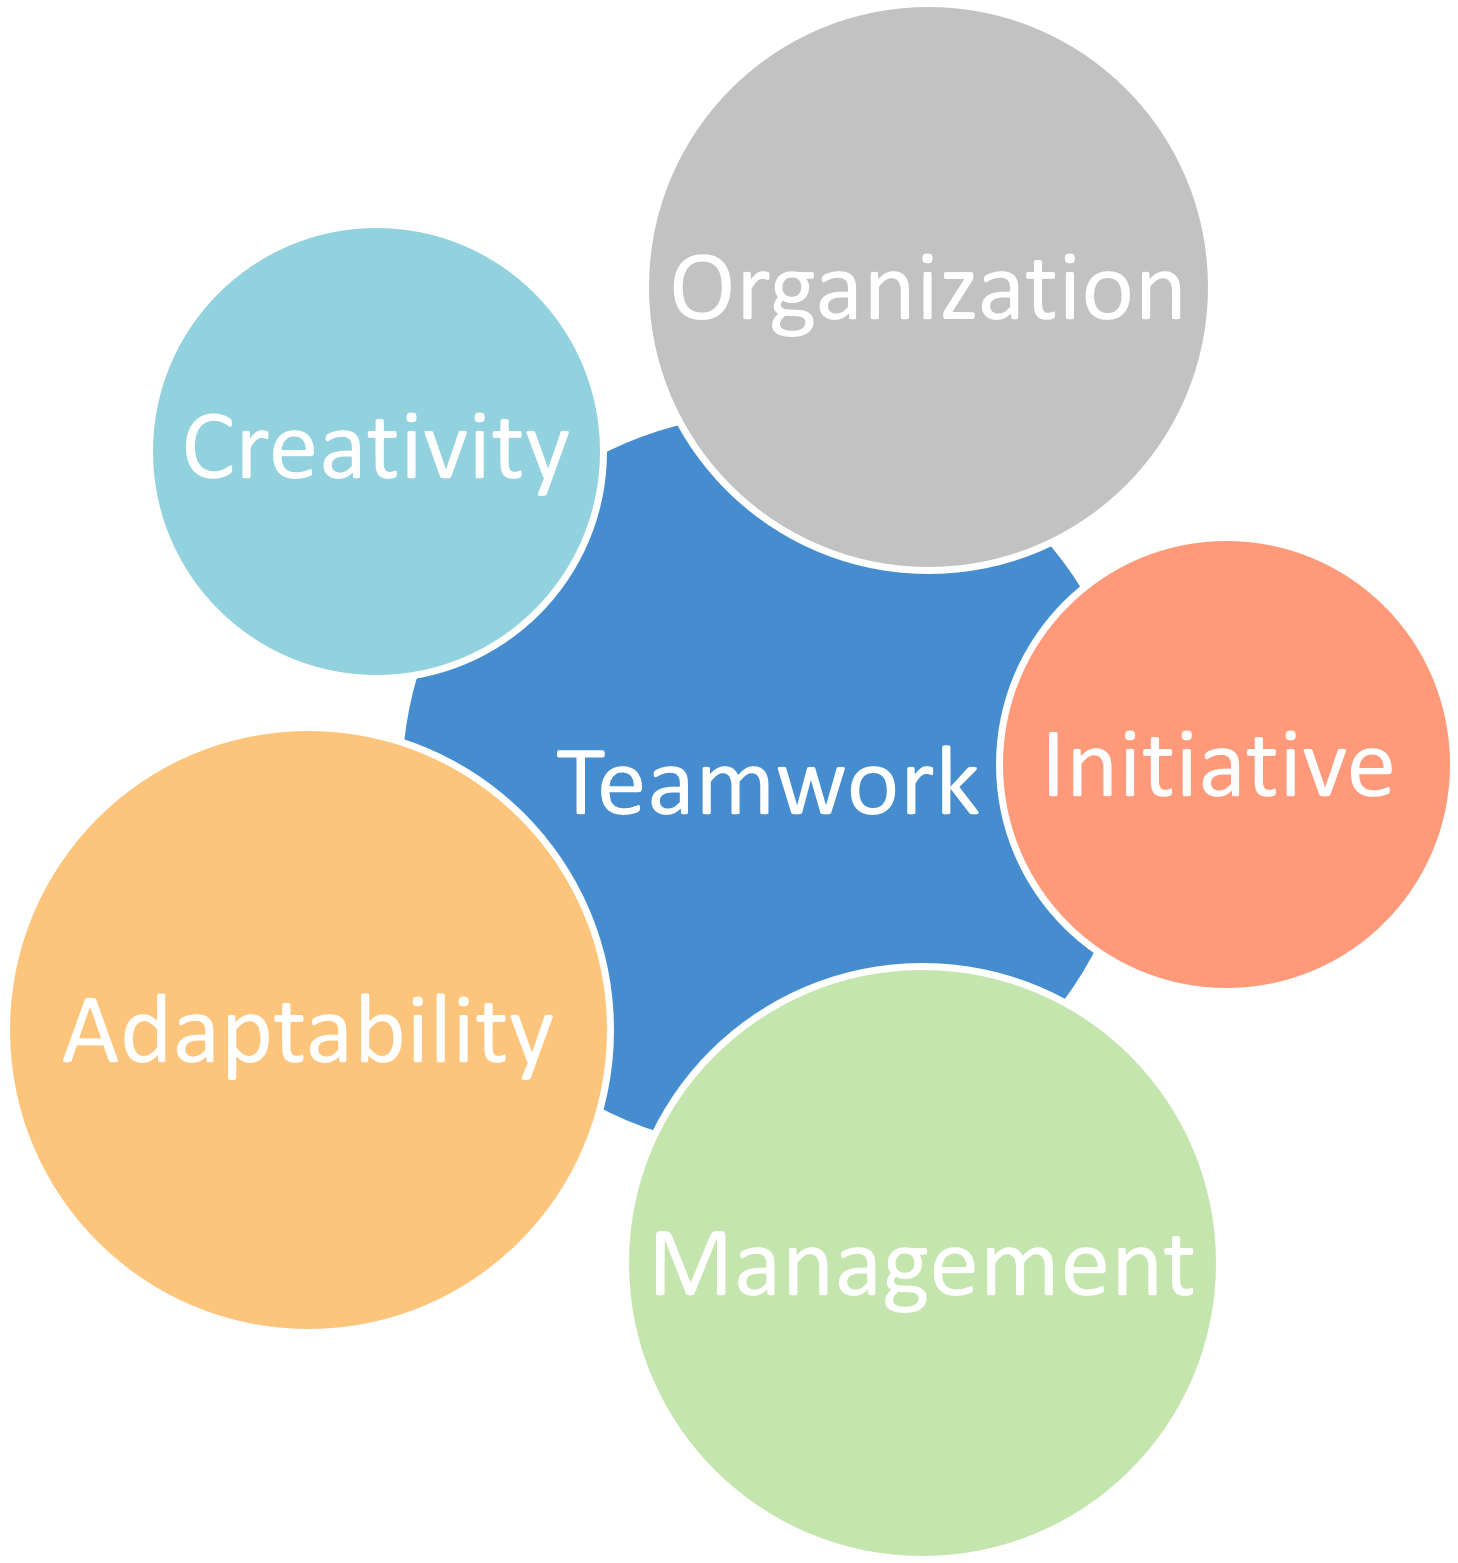
\includegraphics[scale=0.40]{res/img/profileMap_EN.png}\vspace{2.5mm}
\section{CAD / CAM}

\includegraphics[scale=0.40]{res/img/5stars.png}\hspace{1.5mm}\textbf{Catia V5\&V6}

\includegraphics[scale=0.40]{res/img/4stars.png}\hspace{1.5mm}\textbf{Creo 4.0}

\includegraphics[scale=0.40]{res/img/3stars.png}\hspace{1.5mm}\textbf{3D Printing}\section{PLM / PDM}

\includegraphics[scale=0.40]{res/img/4stars.png}\hspace{1.5mm}\textbf{NewPDM}

\includegraphics[scale=0.40]{res/img/3stars.png}\hspace{1.5mm}\textbf{Windchill}\section{FEM / CAE}

\includegraphics[scale=0.40]{res/img/3stars.png}\hspace{1.5mm}\textbf{Ansys Wbench}

\includegraphics[scale=0.40]{res/img/3stars.png}\hspace{1.5mm}\textbf{Abaqus}

\includegraphics[scale=0.40]{res/img/2-5stars.png}\hspace{1.5mm}\textbf{Hyperworks}

\includegraphics[scale=0.40]{res/img/2-5stars.png}\hspace{1.5mm}\textbf{Hypermesh}
\vspace{2.5mm}%\begin{flushleft}
	\emph{Le 12/6/2024} \hspace*{8mm}
	%\end{flushleft}
\end{aside}
\section{IT-Skills}
        \vspace*{-0.45cm}
        \setlength{\columnsep}{-0.3cm}
        \begin{flushleft}
        \begin{multicols}{3}
		\begin{itemize}
		
		\setlength{\itemsep}{5pt}
  		\setlength{\parskip}{0pt}
  		\setlength{\parsep}{0pt}
          
        
\item \large Mobile Development \
\normalsize
\begin{flushleft}


\includegraphics[scale=0.40]{res/img/4stars.png}\hspace{1.5mm}\textbf{Kotlin}\\Room, Firebase, Gson, Jetpack Compose, Retrofit, MVVM, Coroutine\\\vspace{2mm}

\includegraphics[scale=0.40]{res/img/4stars.png}\hspace{1.5mm}\textbf{Flutter}

\includegraphics[scale=0.40]{res/img/4stars.png}\hspace{1.5mm}\textbf{Android}
\end{flushleft}            

\item \large Web Development \
\normalsize
\begin{flushleft}


\includegraphics[scale=0.40]{res/img/4stars.png}\hspace{1.5mm}\textbf{HTML,CSS}

\includegraphics[scale=0.40]{res/img/4stars.png}\hspace{1.5mm}\textbf{JavaScript}
\end{flushleft}            

\item \large Web Frameworks \
\normalsize
\begin{flushleft}


\includegraphics[scale=0.40]{res/img/4stars.png}\hspace{1.5mm}\textbf{Django}

\includegraphics[scale=0.40]{res/img/4stars.png}\hspace{1.5mm}\textbf{Vue.Js}

\includegraphics[scale=0.40]{res/img/3stars.png}\hspace{1.5mm}\textbf{PHP-Laravel}
\end{flushleft}            

\columnbreak
\item \large Back-end / Server \
\normalsize
\begin{flushleft}


\includegraphics[scale=0.40]{res/img/5stars.png}\hspace{1.5mm}\textbf{Python}\\Flask, SQLAlchemy, PyMongo, PyTest, FastAPI, Numpy\\\vspace{2mm}

\includegraphics[scale=0.40]{res/img/3stars.png}\hspace{1.5mm}\textbf{Java}

\includegraphics[scale=0.40]{res/img/3stars.png}\hspace{1.5mm}\textbf{Nginx}

\includegraphics[scale=0.40]{res/img/3stars.png}\hspace{1.5mm}\textbf{Apache}

\includegraphics[scale=0.40]{res/img/4stars.png}\hspace{1.5mm}\textbf{API}
\end{flushleft}            

\item \large Authentication \
\normalsize
\begin{flushleft}


\includegraphics[scale=0.40]{res/img/4stars.png}\hspace{1.5mm}\textbf{JWT Auth}

\includegraphics[scale=0.40]{res/img/3stars.png}\hspace{1.5mm}\textbf{OAuth}

\includegraphics[scale=0.40]{res/img/4stars.png}\hspace{1.5mm}\textbf{Firebase}
\end{flushleft}            

\item \large Devops, CI/CD \
\normalsize
\begin{flushleft}


\includegraphics[scale=0.40]{res/img/4stars.png}\hspace{1.5mm}\textbf{Git / GitLab}

\includegraphics[scale=0.40]{res/img/3stars.png}\hspace{1.5mm}\textbf{Docker}

\includegraphics[scale=0.40]{res/img/3stars.png}\hspace{1.5mm}\textbf{Jenkins}

\includegraphics[scale=0.40]{res/img/3stars.png}\hspace{1.5mm}\textbf{Selenium}

\includegraphics[scale=0.40]{res/img/3stars.png}\hspace{1.5mm}\textbf{Cron}
\end{flushleft}            

\columnbreak
\item \large Databases \
\normalsize
\begin{flushleft}


\includegraphics[scale=0.40]{res/img/4stars.png}\hspace{1.5mm}\textbf{MySQL}

\includegraphics[scale=0.40]{res/img/3stars.png}\hspace{1.5mm}\textbf{PostgreSQL}

\includegraphics[scale=0.40]{res/img/4stars.png}\hspace{1.5mm}\textbf{MongoDB}

\includegraphics[scale=0.40]{res/img/3stars.png}\hspace{1.5mm}\textbf{SQLite}
\end{flushleft}            

\item \large Data \
\normalsize
\begin{flushleft}


\includegraphics[scale=0.40]{res/img/4stars.png}\hspace{1.5mm}\textbf{Shiny}

\includegraphics[scale=0.40]{res/img/4stars.png}\hspace{1.5mm}\textbf{Pandas}

\includegraphics[scale=0.40]{res/img/4stars.png}\hspace{1.5mm}\textbf{Matplotlib}

\includegraphics[scale=0.40]{res/img/4stars.png}\hspace{1.5mm}\textbf{Jupyter}
\end{flushleft}            

\item \large AI \& Tools \
\normalsize
\begin{flushleft}


\includegraphics[scale=0.40]{res/img/3stars.png}\hspace{1.5mm}\textbf{Tensorflow}

\includegraphics[scale=0.40]{res/img/3stars.png}\hspace{1.5mm}\textbf{Keras}
\end{flushleft}            

\item \large Others \
\normalsize
\begin{flushleft}


\includegraphics[scale=0.40]{res/img/3stars.png}\hspace{1.5mm}\textbf{Bash}

\includegraphics[scale=0.40]{res/img/4stars.png}\hspace{1.5mm}\textbf{OpenAPI}

\includegraphics[scale=0.40]{res/img/4stars.png}\hspace{1.5mm}\textbf{Jira}
\end{flushleft}            


        \end{itemize}
        \end{multicols}
        %\end{itemize}
        \end{flushleft} \normalsize
        \vspace*{-0.65cm}
\section{Work Experience}
\vspace*{-0.25cm}

\begin{entrylist}
  \entry
    {09/22 - 11/23}
    {Web \& mobile developer}
    {Synapsun, \textit{Lyon, FR}}
    {Full stack web \& Android mobile developments: \hspace*{8mm}Flutter, Python, Kotlin}
\end{entrylist}
\vspace{-10pt}
\begin{minipage}[t]{0.65\linewidth}
\underline{Context - Mission: }\\
Automate and improve company's repowering* service reactivity (*: Identify and offer replacement solar panels to solar plant owners whose panels are either ageing or damaged\\
\end{minipage} % no space if you would like to put them side by side
\begin{minipage}[t]{0.38\textwidth}
    \underline{Tech. Envir.: }\
    \vspace{1mm}
    
\underline{\textit{Mobile}}: Android, Flutter, Kotlin\\
\underline{\textit{Web}}: Python, Django, Javascript, PHP, HTML, CSS\\
\underline{\textit{Devops, CI/CD}}: Git, GitLab\\
\underline{\textit{Databases}}: PostgreSQL, MongoDB\\
\underline{\textit{Languages}}: French, English (international team)\\
\underline{\textit{Others}}: OpenAPI, API, Jira, VBA
    \end{minipage}
\vspace{1.5mm}
\underline{Goal: }\\

\begin{itemize}
\setlength{\itemsep}{1pt}
\setlength{\parskip}{0pt}
\setlength{\parsep}{0pt}

\item Relieve commercial service in the process dealing with repowering quotation requests and reduce reply time to potential clients.
\item Identify and immediately access client's plant's panels' specifications
\item Automate the search for compatible panels available either in our shop or at suppliers.
\item Give our clients a mobile app whose objective is to guide them to send a quotation request on identified compatible products.
\end{itemize}

\vspace{1.5mm}
\underline{Tasks - Achievements: }\\

\begin{itemize}
\setlength{\itemsep}{1pt}
\setlength{\parskip}{0pt}
\setlength{\parsep}{0pt}

\item Collection of needs, built specification dossier with technical and functional specifications, software application components definition \& design to best answer the company's needs.
\item Web Scraper Development in Python
\item Data Models Design
\item Wrote APIs specifications in the OpenAPI / Swagger standard
\item MongoDB product database and Python FastAPI API setup
\item Mobile Multi-platform client app development in Flutter.
\item Secure Access management with JWT tokens (Json Web Token)
\item PostgreSQL database and Python Django back-end setup for Users and Quotations management.
\item Supplier / Subcontractor contact for outsourced tasks
\end{itemize}

\begin{entrylist}
  \entry
    {11/19 - 04/22}
    {R\&D Engineer}
    {Böllhoff (via Davricourt), \textit{Chambéry, FR}}
    {Automotive Mechatronic Product design \& development}
\end{entrylist}
\vspace{-10pt}
\begin{minipage}[t]{0.65\linewidth}
\underline{Context - Mission: }\\
R\&D Innovation Service, development of a new range of products with high value - instrumented assembly systems and fasteners.\\
\end{minipage} % no space if you would like to put them side by side
\begin{minipage}[t]{0.38\textwidth}
    \underline{Tech. Envir.: }\
    \vspace{1mm}
    
\underline{\textit{CAD}}: DS Catia V5, PTC Creo 7\\
\underline{\textit{PDM}}: Windchill\\
\underline{\textit{CAE}}: Ansys Workbench, Creo Simulate, Altair Simsolid\\
\underline{\textit{DOE, Statistics}}: Minitab\\
\underline{\textit{Extensometry, Acquisition}}: HBM Strain Gauges, Catman Easy, Kickstart Multimeter Oscilloscope\\
\underline{\textit{Languages}}: French, English (international team)\\
\underline{\textit{Others}}: Excel, Powerpoint, VBA
    \end{minipage}
\vspace{1.5mm}
\underline{Tasks - Achievements: }\\

\begin{itemize}
\setlength{\itemsep}{1pt}
\setlength{\parskip}{0pt}
\setlength{\parsep}{0pt}

\item Products and Process/Trials related products design (geometry, CAD/CAE, dimensioning, optimization, interfaces): Sensors, Preconstraint screwed assemblies, Body-fixed elements (tank, roofbox,...), Automotive suspension/Ground liaison elements (McPherson, Flexible, Blade,..), Custom Machines (glueing, pneumatic prehension/command)
\item Technical drawing, Functional dimensioning, Chains of dimensions (Arithmetic, Quadratic)
\item Ensure plays with environment (architectural, thermal, ...)
\item Ensure mountability, positioning and fixation of parts with assembly means
\item Writing trial and validation procedures: Lab, Sub-system, System, Flexion and Tensile trials.
\item Taguchi/Design-Of-Experiments : Definition, Analysis
\item Extensometry, Acquisition: check mechanical resistance and concordance with CAE simulations with strain gauges (HBM)
\item Plasturgy : Water/Dust proof casing design
\item 3D Prototyping: FDM 3D printing, Supplier Contact for other prototype parts
\item Take part in design review meetings : progress and problems sharing, action plan definition and realization.
\end{itemize}

\begin{entrylist}
  \entry
    {11/16 - 09/19}
    {Automotive Design Engineer}
    {Renault (via Bertrandt), \textit{Vélizy, FR}}
    {Underbody \& Engine Compartment Design \& Architecture}
\end{entrylist}
\vspace{-10pt}
\begin{minipage}[t]{0.65\linewidth}
\underline{Context - Mission: }\\
Architecture/Powertrain Service- Vehicle parts design: \\11/16>03/17: Renault Zoé Ph.2 (EV) Engine compartment/Underbody Design/archi;\\08/17>07/19: PHEV, CMF1/CMF-B Platforms, Underbody Design-archi and Technical Management;\\04/19>09/19: Euro7 \& HEV, CD1 Utility Vehicle Platform, Underbody Design-archi and Technical management.\\
\end{minipage} % no space if you would like to put them side by side
\begin{minipage}[t]{0.38\textwidth}
    \underline{Tech. Envir.: }\
    \vspace{1mm}
    
\underline{\textit{CAD}}: DS Catia V6\\
\underline{\textit{PDM}}: NewPDM\\
\underline{\textit{Languages}}: French, English (international team)\\
\underline{\textit{Others}}: Excel, Powerpoint, VBA
\vspace{15mm}
    \end{minipage}
\vspace{1.5mm}
\underline{Tasks - Achievements: }\\

\begin{itemize}
\setlength{\itemsep}{1pt}
\setlength{\parskip}{0pt}
\setlength{\parsep}{0pt}

\item Product definition (Geometry, Interfaces): All kind of part in designated architecture area.
\item Ensure plays with environment (Archi, Thermal,...) with fixed or moving parts
\item Ensure mountability, positioning and fixation of parts with manual or automatic means
\item Technical Drawing, Functional dimensioning, Chains of dimensions (Arithmetic, Quadratic)
\item Design convergence management
\item Team management (Management of French and off-site designers)
\item Organize and lead design review meetings, problem presentations, action plan definition and application.
\end{itemize}

\vspace*{-0.5cm}
\vspace*{0.45cm}
\section{Education - Certifications}
\vspace*{-0.25cm}
\vspace{0.5mm}
\begin{entrylist}
  \entry
    {09/22 - 08/23}
    {Bachelor Degree in Software Design \& Development}
    {EPSI, \textit{Lyon, FR}}
    {RNCP Lvl.6 - Data/IA minor; \hspace{7mm} 09/23: Government Skill Certification}
\end{entrylist}
\vspace*{-0.65cm}
\begin{itemize}
\setlength{\itemsep}{1pt}
\setlength{\parskip}{0pt}
\setlength{\parsep}{0pt}
\begin{multicols}{2}
\item Development: \newline Java, Python, Dart/Flutter, etc.
\columnbreak
\item Data, Databases, etc.
\item Tests \& CI/CD
\end{multicols}
\end{itemize}\vspace{0.5mm}
\begin{entrylist}
  \entry
    {06/22 - 08/22}
    {Web Developer Formation}
    {Epitech, \textit{Paris, FR}}
    {RNCP Lvl.5}
\end{entrylist}

\vspace*{-0.35cm}
\begin{itemize}
\setlength{\itemsep}{1pt}
\setlength{\parskip}{0pt}
\setlength{\parsep}{0pt}

\item PHP, HTML, CSS, JavaScript, Vue.Js, Laravel, Bash, Git
\end{itemize}\vspace{0.5mm}
\begin{entrylist}
  \entry
    {09/13 - 08/16}
    {Master degree in Mechanical Systems Engineering}
    {UTT, \textit{Troyes, FR}}
    {RNCP Lvl.7; Environmental Design \& Industrialization minor}
\end{entrylist}
\vspace{0.5mm}
\begin{entrylist}
  \entry
    {09/11 - 06/13}
    {2-Year Degree in Mechanical Engineering}
    {IUT, \textit{Troyes, FR}}
    {RNCP Lvl.5}
\end{entrylist}
\vspace*{-0.4cm}
\begin{itemize}
\setlength{\itemsep}{1pt}
\setlength{\parskip}{0pt}
\setlength{\parsep}{0pt}
\item Design, Functional dimensioning, enslavement and programming of a robot to take part in the Franch robotic cup.
\end{itemize}
\section{Hobbies}
\vspace*{-0.45cm}
\setlength{\columnsep}{-2cm}
\begin{multicols}{2}
\begin{itemize}
\setlength{\itemsep}{1pt}
\setlength{\parskip}{0pt}
\setlength{\parsep}{0pt}
\item Outings: \\
Hiking, Concerts,  Motorcycle, Photo\\
\item Music: \\
Drums, Piano\\
\columnbreak
\item Travels: \\
Sweden, Cambodia, Thaïland, Germany\\
\item Reading: \\
B.Werber, M.Chattam, F.Thilliez
\end{itemize}
\end{multicols}
\end{document}